% Results section; every number is a macro generated by src/analysis.py
\subsection{The status quo in the data}\label{sec:sq}
Before optimizing, we ask what the city has actually been doing. \Cref{fig:sq}a tabulates the
\NReplaced{} replacements completed in 2021--2025 and the \NRefused{} refusals of access by SVI
quintile. Two facts emerge. First, recent replacement activity has been mildly progressive: \ReplQE{}
replacements per 1,000 lines requiring action in the most vulnerable quintile against \ReplQA{} in the
least, consistent with the city's income-qualified Equity program and block work along main
replacements. The common presumption that request-driven programs are regressive does not describe
Chicago's recent record. Second, refusals rise steeply with vulnerability, from \RefQA{} to \RefQE{}
per 1,000 lines, tracking renter share (\RentQA\% to \RentQE\%). \Cref{sec:consent} shows that this
gradient survives controls. The equity problem in the data is therefore less about whom the city
chooses to serve than about whom it can reach.

\begin{figure}[t]\centering
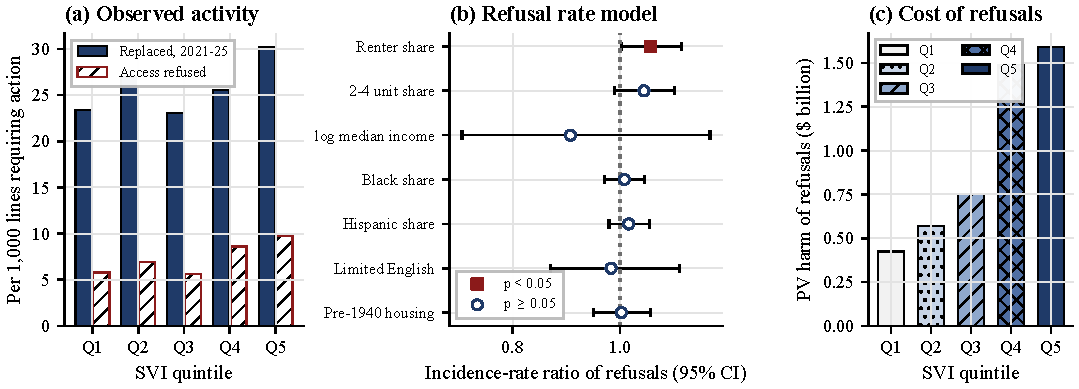
\includegraphics[width=\linewidth]{fig05_status_quo.pdf}
\caption{The status quo in the 2025 inventory. (a) Completed replacements (2021--2025) and refusals of access per 1,000 lines requiring action, by SVI quintile of the zone. (b) Incidence-rate ratios (95\% CI, standard errors clustered by community area) from a negative-binomial model of refusals per line across 608 tracts. (c) PV harm attributable to refusals under the health-welfare schedule, assuming refused lines wait until 2046. Recent replacements were mildly progressive, but refusals rise with vulnerability and renter share and concentrate the cost of refusals in the most vulnerable quintiles.}\label{fig:sq}
\end{figure}

\subsection{Scenario comparison}
We compare eight schedules (\cref{tab:scen}), all evaluated on a common yardstick (central harm,
$r=3\%$). Three are heuristics on the same budget and crew path: the \emph{status quo}, which allocates
capacity in proportion to each zone's empirical-Bayes smoothed 2021--2025 replacement rate;
\emph{proportional pace}, which advances every zone at the same rate; and \emph{harm priority}, which
fills capacity in descending $h_z$. All three use one-off delivery, because spreading crews across
the city never reaches block batch sizes; repricing the status quo with block pricing wherever a
zone-year reaches $m_z$ changes its cost by less than \$0.02 billion. Five are MILP solutions:
cost-minimizing (CM, $\alpha_H=0$), health-welfare (HW), equity-weighted with linear and convex SVI
weights (EW, EW-convex) and distributional weights (DW). All MILPs impose the EJ floor.

\begin{table}[t]\centering\scriptsize
\caption{Scenario outcomes ($r=3\%$; PV in \$ billion; waits are expected replacement years,
$t=1$ is 2027). $G$ is the Q5 wait gap (\cref{eq:eps}); $C$ is the concentration index of residual
child exposure ranked by SVI (negative = burden on the less vulnerable); $\mathcal G$ is the Gini of
exposure. Gap is the solver's absolute optimality gap (\$ million).}\label{tab:scen}
\setlength{\tabcolsep}{3pt}
\begin{tabular}{@{}lccccccccccc@{}}
\toprule
Schedule & PV $H$ & PV $C$ & PV $H{+}C$ & Done & $\bar W_{\EJ}$ & $\bar W_{\neg\EJ}$ & $G$ & $C$ & $\mathcal G$ & Block\,\% & Gap\\
\midrule
\csname @@input\endcsname tab_scenarios.tex 
\bottomrule
\end{tabular}
\end{table}

The status quo replaces \SQDonePct\% of the inventory by 2046 and finishes in \SQCompletion, missing
the deferred LCRI deadline. Its PV social cost is \$\SQSocial{} billion. The health-welfare schedule
finishes on time at \$\HWSocial{} billion, a saving of \$\DecTotal{} billion (\GainPct\%), of which
\$\DecHarmTotal{} billion is avoided harm and \$\DecCostTotal{} billion discounted capital. Nominal
capital spending falls from \$\SQNominal{} to \$\HWNominal{} billion. No one-off schedule can meet the
deadline at all: with block programs disabled the HW problem is infeasible, because 412,433 one-off
replacements at \$39,000 cost \$16.1 billion against \$\TotalBudget{} billion of capital over the
horizon.

One caveat on pricing deserves emphasis. The city's reported overall average (\$31,000) is below
both its block (\$34,000) and one-off (\$39,000) averages, which implies cheaper categories of work
within the current mix. If the status quo is priced at \$31,000 per line instead of the one-off rate,
its PV cost falls to \$\SQAltCost{} billion and its social cost to \$\SQAltSocial{} billion; the
health-welfare schedule still saves \$\SavingAlt{} billion (\SavingAltPct\%), now driven almost
entirely by avoided harm. The ordering result is robust to this choice; the size of the clustering
gain is not, and it should be re-estimated from CDWM contract data.

The saving decomposes cleanly. Moving from the status quo to harm priority with the same one-off
delivery saves \$\DecOrdering{} billion (\DecOrderPct\%): this is the value of ordering by risk.
Moving from harm priority to the HW solution saves a further \$\DecClustering{} billion
(\DecClusterPct\%): this is the value of clustering work into block programs and timing
mobilizations, which also lets the program finish on time. The cost-minimizing schedule captures
most of the clustering value but ignores harm and therefore leaves \$\CMHarm{} billion of PV harm
against \$\HWHarm{} billion under HW.

\subsection{Who is served first, and where}
\Cref{fig:sched} shows annual replacements by SVI quintile and \cref{fig:cmap} maps each zone's
expected replacement year. The status quo spreads capacity almost uniformly, so every zone waits
about the same (\SQWaitEJ{} years in EJ zones against \SQWaitNonEJ{} elsewhere). HW concentrates early
capacity on the West and Southwest Sides, where child density and confirmed lead are highest,
then moves outward; low-harm lakefront zones, dominated by large buildings with few small-diameter
lead services, come last. EJ zones are half complete by 2033, 84\% by 2039 and fully replaced by 2044 under HW
(\cref{fig:paths}), and
their expected replacement year is \HWWaitEJ{} against \HWWaitNonEJ{} for other zones.
Consistent with \cref{prop:smith}, the HW order tracks $h_z$, and because $h_z$ rises with SVI
(\cref{fig:damage}c), it is progressive without being told to be.

\begin{figure}[t]\centering
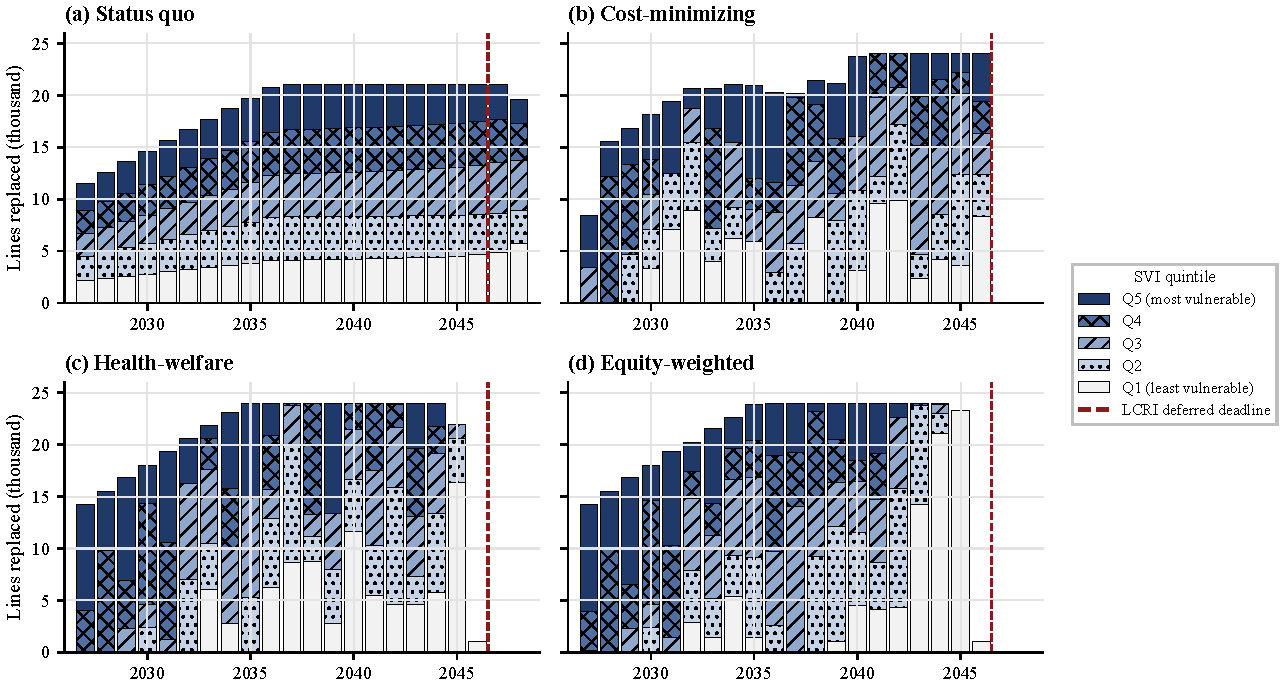
\includegraphics[width=\linewidth]{fig06_schedules.pdf}
\caption{Annual replacements by SVI quintile under four schedules: the empirical status quo (heuristic based on 2021--2025 replacement rates) and three MILP solutions (cost-minimizing, health-welfare and equity-weighted), all under the same budget and crew limits. The dashed line marks the end of the deferred LCRI schedule. The status quo spreads capacity evenly and misses the deadline, whereas the health-welfare schedule serves the most vulnerable quintile first and finishes on time.}\label{fig:sched}
\end{figure}

\begin{figure}[t]\centering
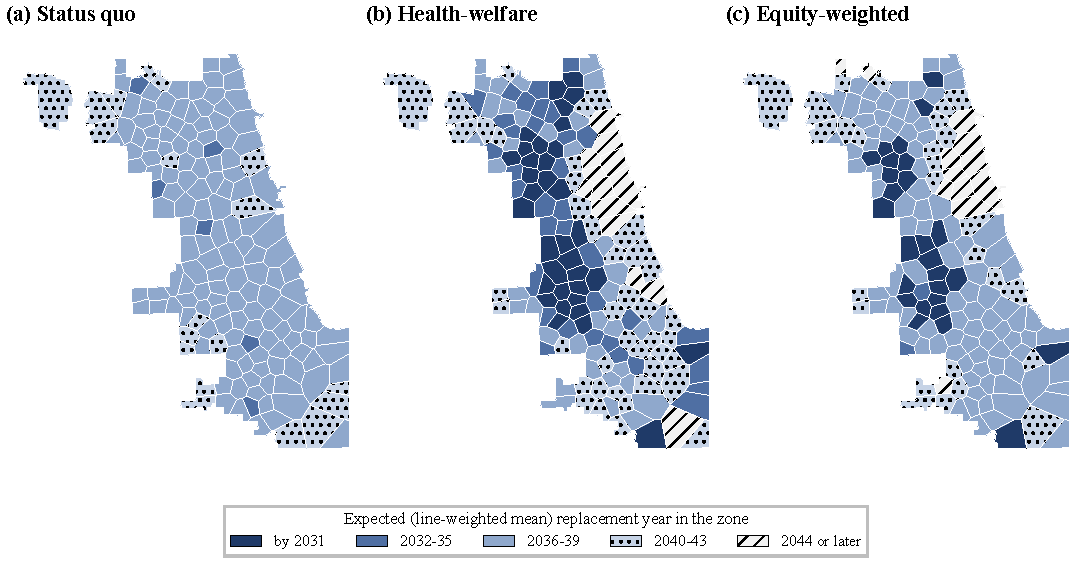
\includegraphics[width=\linewidth]{fig07_completion_maps.pdf}
\caption{Expected (line-weighted mean) replacement year of each of the 160 zones under the status quo, health-welfare and equity-weighted schedules; zones are Voronoi cells around the centroids of k-means clusters of lines requiring action. Optimized schedules replace the West and Southwest Sides first and the low-harm lakefront last, while the status quo leaves nearly every zone waiting until the late 2030s.}\label{fig:cmap}
\end{figure}

\begin{figure}[t]\centering
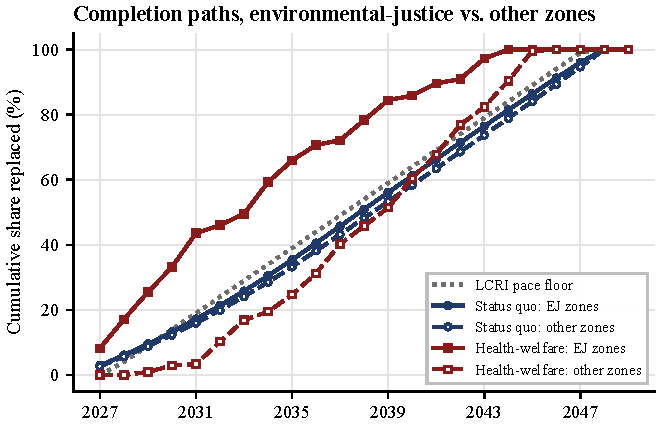
\includegraphics[width=0.7\linewidth]{fig08_completion_paths.pdf}
\caption{Cumulative share of lines replaced in environmental-justice zones (SVI at or above the 60th percentile) and other zones, status quo against the health-welfare schedule, with the LCRI pace floor. Under the health-welfare schedule EJ zones are half complete by 2033 and fully replaced by 2044, about four years before the status quo finishes them in 2048.}\label{fig:paths}
\end{figure}

\subsection{The welfare--equity frontier}
\Cref{fig:frontier} plots PV social cost against the Q5 gap. Three results stand out.

\emph{First, the welfare optimum is already progressive.} HW serves the most vulnerable quintile
\HWGapAbs{} years earlier than the citywide mean ($G=\HWGap$). Pricing harm correctly and serving the vulnerable first
are the same instruction over most of the range.

\emph{Second, delaying the vulnerable is dominated.} Every schedule to the right of HW, including the
reversed-constraint solutions with the EJ floor removed, has higher social cost and a worse gap. The
status quo and proportional pace sit far above and to the right of the frontier: no ethical weighting
that values both welfare and vertical equity would choose them over HW.

\emph{Third, along the frontier the trade-off is real but cheap.} Pushing $G$ from \HWGap{} to
\FrontMinGap{} years costs \$\FrontMinGapCost{} billion, under 2\% of social cost; beyond about $-8$
years the problem is infeasible under the capacity and pace constraints. Moving in the regressive
direction is also cheap (forcing $G=0$ costs \$\DomZeroCost{} billion), which is why equity cannot be
left to welfare arithmetic alone: the penalty for a regressive schedule is small enough that
administrative convenience could easily outweigh it. The EJ floor \eqref{c:ej} makes the
progressive ordering binding rather than merely optimal. The more consequential numbers lie off the
frontier: the \$\DecTotal{} billion between the status quo and HW, and the \$\RefCost{} billion cost of
refusals (\cref{sec:consent}).

\begin{figure}[t]\centering
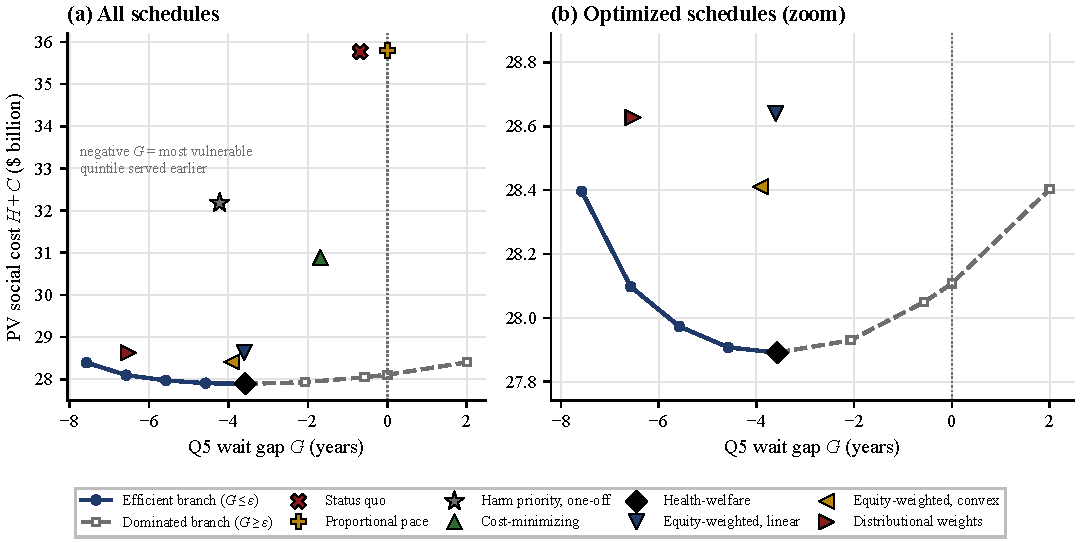
\includegraphics[width=\linewidth]{fig09_frontier.pdf}
\caption{Welfare--equity frontier traced with the $\varepsilon$-constraint method: each point on the efficient branch minimizes PV social cost subject to a bound on the Q5 wait gap $G$, and the dominated branch forces $G\geq\varepsilon$ with the EJ floor relaxed; markers show heuristic and MILP scenarios evaluated at central parameters and $r=3\%$. Panel (b) enlarges the optimized schedules. The welfare optimum is already progressive, schedules that delay the most vulnerable are dominated, and additional priority costs less than 2\% of social cost.}\label{fig:frontier}
\end{figure}

\subsection{Five equity frameworks}
The frameworks embed different normative commitments, and the data show how much those commitments
matter in practice. (i) \emph{Utilitarian} HW is progressive through the correlation of harm and
vulnerability. (ii) \emph{Distributional weights} with $\eta=1$ reweight harm toward low-income zones
and produce the most progressive schedule ($G=\DWGap$; EJ zones wait \DWWaitEJ{} years) at
\$\DWSocial{} billion on the utilitarian yardstick, \$0.74 billion above HW. (iii) The
\emph{linear SVI penalty} (EW) barely changes the Q5 gap ($G=\EWGap$) but lowers dispersion
(Atkinson $A_1$ from \HWAtkOne{} to \EWAtkOne): because \cref{eq:E} charges any zone that waits longer
than average and moderate-SVI zones carry substantial weight, it acts largely as a horizontal-equity
term that compresses waits. (iv) The \emph{convex SVI penalty} (EW-convex) concentrates weight on the
most vulnerable and moves $G$ to \ECGap{} at lower cost than EW. (v) The \emph{Rawlsian} limit, the
leftmost feasible frontier point, gives the most vulnerable quintile the maximum feasible priority
($G=\FrontMinGap$). The lesson for practice is that the functional form of an equity term is a
normative choice, not a technicality: a linear vulnerability-weighted penalty buys horizontal
equality, whereas distributional weights or convex weights buy priority for the worst off.

\subsection{The inequality-index paradox}\label{sec:paradox}
The symmetric inequality indices in \cref{tab:scen} rank the schedules almost exactly backwards.
Proportional pace has a Gini of zero and the status quo nearly so (\SQGini), while HW has the
highest Gini (\HWGini) and harm priority the highest Atkinson index (\POAtkOne). Gini and Atkinson
measure dispersion, and the status quo achieves low dispersion by delaying everyone, including the
most exposed, at a similar rate. Triage is unequal treatment of unequal risk, and a symmetric index
cannot tell progressive from regressive inequality.

Directional measures resolve the paradox. \Cref{fig:conc} plots concentration curves of residual
child exposure-years with children ordered from most to least vulnerable \citep{wagstaff1991}. The
status quo lies on the diagonal ($C=\SQConc$); HW lies well below it ($C=\HWConc$), so the most
vulnerable children bear much less than their population share of remaining exposure. An
algorithmic-equity audit that relies on Gini or Atkinson indices alone would penalize exactly the
triage that environmental justice calls for. Audits should report a directional statistic: the gap
$G$, a concentration index, or completion paths by vulnerability.

\begin{figure}[t]\centering
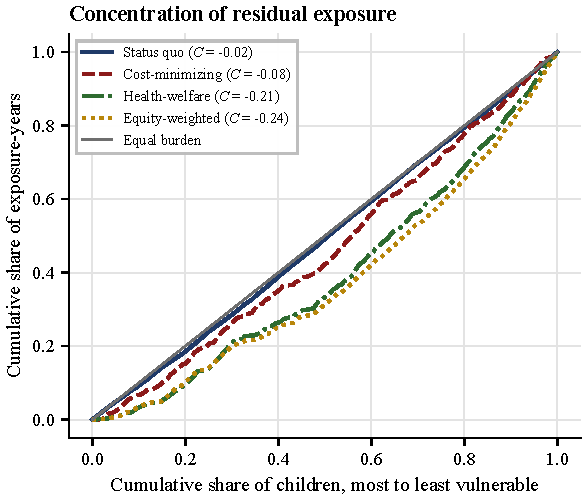
\includegraphics[width=0.6\linewidth]{fig10_concentration.pdf}
\caption{Concentration curves of residual child exposure-years, computed from each schedule's yearly replacement shares and zone child density, with children ordered from most to least vulnerable; $C$ is the concentration index. The status quo spreads remaining exposure almost evenly ($C\approx0$), whereas optimized schedules place it on the less vulnerable, which symmetric Gini and Atkinson indices fail to distinguish.}\label{fig:conc}
\end{figure}

\subsection{Robustness of the schedule}\label{sec:robust}
\Cref{tab:robust} re-solves HW under alternative discount rates, benefit tiers and a tap-lead
gradient taken from \citet{huynh2024}. The schedule itself is remarkably stable. Evaluated on the
common yardstick, every variant is within \$0.3 billion of HW, and the Q5 gap ranges only from
\HChGap{} to \HHuGap{} years. The discount rate barely moves the order because zones holding more than 99\% of lines
have harm above the \cref{prop:delay} threshold even at 7\%, so budgets rather than discounting
determine timing. The tap-lead gradient, which raises harm in heavily Hispanic zones on the Southwest Side,
moves some of those zones earlier and narrows the gap, a reminder that better exposure data could
reorder the middle of the schedule. What is uncertain is the size of the benefits, not the sequence.

\begin{table}[t]\centering\small
\caption{Robustness of the health-welfare schedule. ``Own'' is PV social cost under the variant's own
assumptions; ``Common'' evaluates the variant's schedule under the central assumptions at 3\%.}
\label{tab:robust}
\begin{tabular}{@{}lcccccc@{}}
\toprule
Variant & Own $H{+}C$ & Common $H{+}C$ & $G$ & $\bar W_{\EJ}$ & $\bar W_{\neg\EJ}$ & Block\,\%\\
\midrule
\csname @@input\endcsname tab_robust.tex 
\bottomrule
\end{tabular}
\end{table}
